% !TEX TS-program = pdflatex
% !TEX encoding = UTF-8 Unicode
% !TEX root = JoshuaPaulBarnards-Resume.tex
% !TEX spellcheck = en-EN
% !BIB program = biber

% Joshua Paul Barnard's LaTeX Resume
%
% Developed on Windows 10, coded and compiled using TeXstudio 4.7.1 and MikTex 23.10, 8678.
% 
% This resume can be downloaded from:
%  https://github.com/JoshuaPaulBarnard/resume
%
% Author:
%  Joshua Paul Barnard <JoshuaPaulBarnard@gmail.com>
%
% References:
%  National Institute of Technology, Warangal <overleaf.com/latex/templates/nit-warangal-resume/gtsrbjvffcjn>
%
% Template license:
%  MIT (https://mit-license.org/)

%---------------------- Required Formatting -----------------------
\documentclass[a4paper, 11pt]{article}
\title{Joshua Paul Barnard's Resume}
\author{Joshua Paul Barnard}

%-------------------------------------------------------------------------------
% REQUIRED PACKAGES
%-------------------------------------------------------------------------------
\usepackage{latexsym}
\usepackage{xcolor}
\usepackage{float}
\usepackage{ragged2e}
\usepackage[empty]{fullpage}
\usepackage{wrapfig}
\usepackage{lipsum}
\usepackage{tabularx}
\usepackage{titlesec}
\usepackage{geometry}
\usepackage{marvosym}
\usepackage{verbatim}
\usepackage{enumitem}
\usepackage[hidelinks]{hyperref}
\usepackage{fancyhdr}
\usepackage{fontawesome5}
\usepackage{multicol}
\usepackage{graphicx}
\usepackage{cfr-lm}
\usepackage[T1]{fontenc}
\usepackage[most]{tcolorbox}


%-------------------------------------------------------------------------------
% CONFIGURATIONS
%-------------------------------------------------------------------------------
\geometry{left=1.4cm, top=0.8cm, right=1.2cm, bottom=1cm}
\setlength{\multicolsep}{0pt} 
\pagestyle{fancy}
\fancyhf{} % clear all header and footer fields
\fancyfoot{}
\renewcommand{\headrulewidth}{0pt}
\renewcommand{\footrulewidth}{0pt}

% Adjust margins
%\addtolength{\oddsidemargin}{-0.5in}
%\addtolength{\evensidemargin}{-0.5in}
%\addtolength{\textwidth}{1in}

\tcbset{
	frame code={}
	center title,
	left=0pt,
	right=0pt,
	top=0pt,
	bottom=0pt,
	colback=gray!20,
	colframe=white,
	width=\dimexpr\textwidth\relax,
	enlarge left by=-2mm,
	boxsep=4pt,
	arc=0pt,outer arc=0pt,
}

\urlstyle{same}

\raggedright
\setlength{\tabcolsep}{0in}


%-------------------------------------------------------------------------------
% Sections formatting
%-------------------------------------------------------------------------------
\titleformat{\section}{
	\vspace{-4pt}\scshape\raggedright\large
}{}{0em}{}[\color{black}\titlerule \vspace{-7pt}]


%-------------------------------------------------------------------------------
% Custom commands
%-------------------------------------------------------------------------------
\newcommand{\resumeItem}[2]{
	\item{
		\textbf{#1}{\hspace{0.5mm}#2 \vspace{-0.5mm}}
	}
}

\newcommand{\resumePOR}[3]{
	\vspace{0.5mm}\item
	\begin{tabular*}{0.97\textwidth}[t]{l@{\extracolsep{\fill}}r}
		\textbf{#1}\hspace{0.3mm}#2 & \textit{\small{#3}} 
	\end{tabular*}
	\vspace{-2mm}
}

\newcommand{\resumeSubheading}[4]{
	\vspace{0.5mm}\item
	\begin{tabular*}{0.98\textwidth}[t]{l@{\extracolsep{\fill}}r}
		\textbf{#1} & \textit{\footnotesize{#4}} \\
		\textit{\footnotesize{#3}} &  \footnotesize{#2}\\
	\end{tabular*}
	\vspace{-2.4mm}
}

\newcommand{\resumeProject}[4]{
	\vspace{0.5mm}\item
	\begin{tabular*}{0.98\textwidth}[t]{l@{\extracolsep{\fill}}r}
		\textbf{#1} & \textit{\footnotesize{#3}} \\
		\footnotesize{\textit{#2}} & \footnotesize{#4}
	\end{tabular*}
	\vspace{-2.4mm}
}

\newcommand{\resumeSubItem}[2]{\resumeItem{#1}{#2}\vspace{-4pt}}

% \renewcommand{\labelitemii}{$\circ$}
\renewcommand{\labelitemi}{$\vcenter{\hbox{\tiny$\bullet$}}$}

\newcommand{\resumeSubHeadingListStart}{\begin{itemize}[leftmargin=*,labelsep=0mm]}
	\newcommand{\resumeHeadingSkillStart}{\begin{itemize}[leftmargin=*,itemsep=1.7mm, rightmargin=2ex]}
		\newcommand{\resumeItemListStart}{\begin{justify}\begin{itemize}[leftmargin=3ex, rightmargin=2ex, noitemsep,labelsep=1.2mm,itemsep=0mm]\small}
				
				\newcommand{\resumeSubHeadingListEnd}{\end{itemize}\vspace{2mm}}
			\newcommand{\resumeHeadingSkillEnd}{\end{itemize}\vspace{-2mm}}
		\newcommand{\resumeItemListEnd}{\end{itemize}\end{justify}\vspace{-2mm}}
\newcommand{\cvsection}[1]{%
	\vspace{2mm}
	\begin{tcolorbox}
		\textbf{\large #1}
	\end{tcolorbox}
	\vspace{-4mm}
}

\newcolumntype{L}{>{\raggedright\arraybackslash}X}%
\newcolumntype{R}{>{\raggedleft\arraybackslash}X}%
\newcolumntype{C}{>{\centering\arraybackslash}X}%
%--------- End of Packages and Formatting ----------



%-------------------------------------------
%%%%%%  CV STARTS HERE  %%%%%%%%%%%
%%%%%% DEFINE ELEMENTS HERE %%%%%%%
\newcommand{\name}{Joshua Paul Barnard} % Your Name

\newcommand{\phone}{(707) 809 - 5409} % Your Phone Number
\newcommand{\emaila}{JoshuaPaulBarnard@gmail.com} %Email 1
\newcommand{\emailb}{JoshuaPaulBarnard.com} %Email 2




\begin{document}
	\fontfamily{cmr}\selectfont
	%----------HEADING-----------------
	
	
	\parbox{2.35cm}{%
		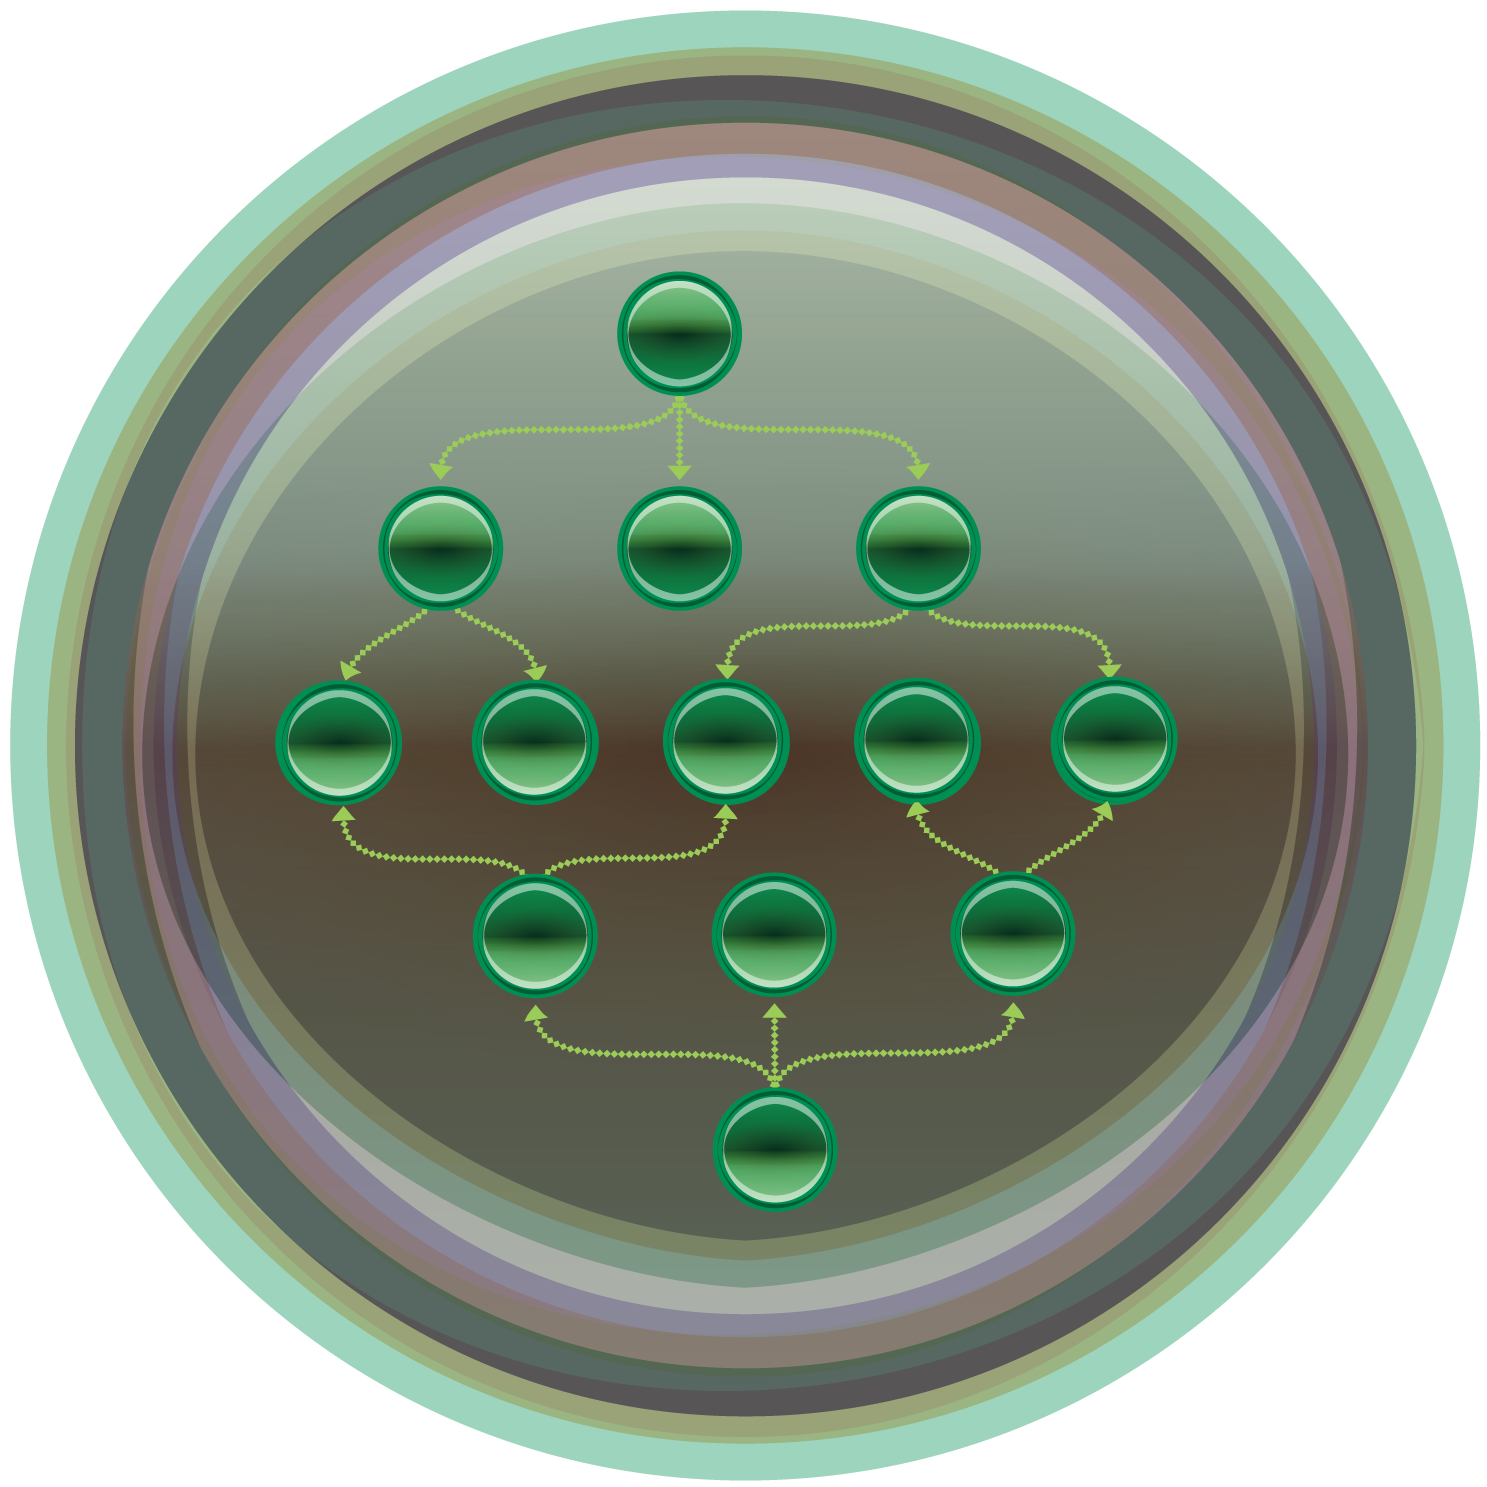
\includegraphics[width=2cm,clip]{LOGO.png}
	}
	\parbox{\dimexpr\linewidth-2.8cm\relax}{
	\begin{tabularx}{\linewidth}{L r} \\
		\textbf{\Large \name} &  \href{https://JoshuaPaulBarnard.com}{\raisebox{0.0\height}{\footnotesize \faGlobe}\ {Portfolio Website}}\\
		{ Northern California } &  \href{https://github.com/JoshuaPaulBarnard}{\raisebox{0.0\height}{\footnotesize \faGithub}\ {GitHub Profile}} \\
		{ JoshuaPaulBarnard@gmail.com } & \href{https://www.linkedin.com/in/joshua-paul-barnard/}{\raisebox{0.0\height}{\footnotesize \faLinkedin}\ {LinkedIn}}
	\end{tabularx}
	}
	% \parbox{3.0cm}{%
		% \flushright \includegraphics[width=2cm,clip]{nitp_logo.png}
		% }
	
	
	
	
	%-----------EDUCATION-----------
	\section{\textbf{Education}}
	\resumeSubHeadingListStart
	\resumeSubheading
	{Johns Hopkins University, Whiting School of Engineering}{}
	{Masters of Science:  Data Science}{2026}
	\resumeSubheading
	{Humboldt State University}{}
	{Bachelors of Art:  Psychology}{2016}
	\resumeSubheading
	{Santa Rosa Junior College}{}
	{Associates of Science:  Computer Science}{2018}
	\resumeSubheading
	{Cornell University, eCornell}{}
	{Certificate:  Data Analytics}{2017}
	\resumeSubHeadingListEnd
	\vspace{-5.5mm}
	%---------------------------------
	
	
	
	%-----------EXPERIENCE-----------------
	\section{\textbf{Experience}}
	\resumeSubHeadingListStart
	
	\resumeSubheading
	{Mendocino College}{Ukiah, CA}
	{Computer Support Technician, Instructor \& Tutor}{2022 - Present}
	\vspace{-1.0mm}
	\resumeItemListStart
	\item {Computer Support Technician:  PC \& Mac Software \& Hardware Repair, TCP/IP \& Networking, IT Support.}
	\item {Computer Science Instructor:  Curriculum Development, Syllabus Creation, Classroom Management.}
	\item {Tutor in Mathematics and Statistics, assisted with Hybrid Classrooms using Zoom Cart.}
	\resumeItemListEnd
	
	\vspace{-3.0mm}
	
	\resumeSubheading
	{Omniworld UK}{London, UK}
	{Lead Developer}{2023 - Present}
	\vspace{-1.0mm}
	\resumeItemListStart
	\item {Developing the Crown Blockchain based on Cryptonote, written in C++ and using Github.}
	\item {Integrating The Crown Coin with Phone App and banking API to provide The Crown Card.}
	\resumeItemListEnd
	
	\vspace{-3.0mm}
	
	\resumeSubheading
	{Sequoidea Properties LLC}{Fort Bragg, CA}
	{Property Manager}{2020 - Present}
	\vspace{-1.0mm}
	\resumeItemListStart
	\item {Performing Regular Maintenance, Handling Tenants Needs,  Accounting, and Ensuring Legal Compliance.}
	\item {Responsibilities range from plumping, logging, and construction, to accounting, research, and systems networking.}
	\resumeItemListEnd
	
	\vspace{-3.0mm}
	
	\resumeSubheading
	{Santa Rosa Junior College}{Santa Rosa, CA}
	{Tutor \& Instructional Assistant}{2001 - 2018}
	\vspace{-1.0mm}
	\resumeItemListStart
%	\item {Group, Drop-In, Lab, Private, and 1-on-1 Tutoring}
	\item {Subjects Included:  Computer Science, Statistics, Web Development, Multimedia, Mathematics, Psychology.}
	\resumeItemListEnd
	
	\resumeSubHeadingListEnd
	\vspace{-8.5mm}
	
	
	
	%-----------PROJECTS-----------------
	\section{\textbf{Projects}}
	\resumeSubHeadingListStart
	
	\resumeProject
	{Predicting Wine Quality by comparing Linear Regression with Machine Learning Techniques.} %Project Name
	{The Johns Hopkins University} %Location, authors, etc
	{2022} %Event Dates
	
	\resumeItemListStart
	\item {Various techniques were used to predict the perceived quality of wine based on physio-chemical properties.}
	\item {Tools Used:  Python, Jupyter, NumPy, Pandas, Seaborn, OBS}
	\resumeItemListEnd
	\vspace{-2mm}
	
	\resumeProject
	{SNAP Cats Website Redesign} %Project Name
	{Santa Rosa Junior College} %Location, authors, etc
	{2018} %Event Dates
	
	\resumeItemListStart
	\item {Project Manager using Agile software development practices, using Slack and Trello. }
	\item {Designed and developed a modern responsive website for a local non-profit using Wordpress(.org).}
	\resumeItemListEnd
	\vspace{-2mm}
	
	\resumeProject
	{Reliability and Validity of the Health Efficacy Scale for College Students} %Project Name
	{Humboldt State University (Cal Poly Humboldt)} %Location, authors, etc
	{2015} %Event Dates
	
	\resumeItemListStart
	\item {16-item scale developed to assesses an individual’s belief in their capacity to change their own health.  }
	\item {Examined the psychometric properties of the HESCS by reliability and validity in SPSS with a sample of 104.}
	\resumeItemListEnd
	\vspace{-2mm}
	
	\resumeSubHeadingListEnd
	\vspace{-5.5mm}
	
	
	%-----------Technical skills-----------------
	\section{\textbf{Technical Skills and Interests}}
	\begin{itemize}[leftmargin=0.05in, label={}]
		\small{\item{
				\textbf{Developer Tools}{: }{ }{ }{ }{ } R, Python, SQL, Linux, Java, TeX, Git, Solidity, Rust, PHP, CSS3, HTML5, C++, JavaScript.\\
				\textbf{Frameworks}{: }{ }{ }{ }{ }{ }{ }{ }{ } TensorFlow, Pandas, Scrapy, Phaser.js, Next.js, Angular, React, D3.js NodeJS. \\
				\textbf{Cloud/Databases}{: }{ }{ }{ } AWS, Google Cloud, Microsoft Azure, MySQL, NoSQL, SQLite, MongoDB.\\
				\textbf{Coursework}{: }{ }{ }{ }{ }{ }{ }{ }{ } Statistical Modeling, Data Science, Psychometrics, Calculus, Predictive Data Analysis.\\
				\textbf{Programs}{: }{ }{ }{ }{ }{ }{ }{ }{ }{ }{ }  Excel, Trello, Tableau, SPSS, Visual Studio Code, Jupyter Notebook, Photoshop, Wordpress.  \\
				\textbf{Soft Skills}{: }{ }{ }{ }{ }{ }{ }{ }{ }{ }{ } Project Management, Attention to Detail, Problem-solving, Adaptability \& Creativity.\\
				\textbf{Experience}{: }{ }{ }{ }{ }{ }{ }{ }{ }{ } Linux Server Administration, Agile Scrum Leader, Education, PC repair tech, IT Support.\\
				\textbf{Areas of Expertise}{: }{ } Statistics, Programming, Web Development, Education, Management. \\
				\textbf{Subjects of Interest}{: } Research, Data Science, Blockchain Development, Artificial Intelligence.\\
		}}
	\end{itemize}
	\vspace{-16pt}
	
	
	
	%-----------Positions of Responsibility-----------------
	\section{\textbf{Positions of Responsibility}}
	\vspace{-0.4mm}
	\resumeSubHeadingListStart
	
	\resumePOR{Founder \& President,  } % Position
	{ HSU Statistics and Probability Club} %Club,Event
	{2014 - 2016} %Tenure Period
	
	\resumeSubHeadingListEnd
	\vspace{-5mm}
	
	
	
	
	%-----------Achievements-----------------
	\section{\textbf{Achievements}}
	\vspace{-0.4mm}
	\resumeSubHeadingListStart
	
	\resumePOR{Eagle Scout,  } % Award
	{   Boy Scouts of America, Troop 37.} % Event
	%{   Earned over 45 Merit Badges \& Restored Braille Trail in County Park.} % Event
	{2004} %Event Year
	
	\resumeSubHeadingListEnd
	\vspace{-5mm}



%-------------------------------------------
\end{document}